\section{Theorie}
\label{sec:theorie}

Als Photoeffekt wird das Auslösen von Elektronen aus einer Metalloberfläche, die mit Licht bestrahlt wird, bezeichnet.
Die Emission von Elektron findet erst statt, wenn die Frequenz des Lichtes die für jedes Metall charakteristische Grenzfrequenz überschreitet.
Trifft ein Photon ein Elektron im Metall, überträgt es seine gesamte Energie auf das Elektron.
Sollte die Energie des Photons größer als die Austrittsarbeit des Metalls sein, wird das Elektron emittiert und die restliche Energie bleibt als kinetische Energie des Elektrons erhalten.
%Treffen Lichtquanten auf eine Metalloberfläche,
%lösen sie, sofern ihre Energie ausreicht, Elektronen aus. \\

Um diesen, auch Photoeffekt genannten Effekt näher zu untersuchen,
kann der in \autoref{fig:abb1} dargestellte Aufbau verwendet werden.

\begin{figure}[H]
    \centering
    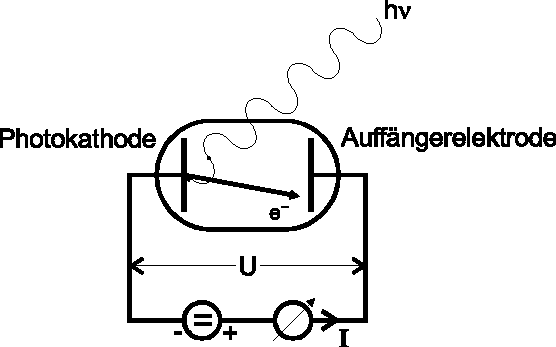
\includegraphics{figures/Abb1.pdf}
    \caption{Aufbau zur Untersuchung des Photoeffekts \cite{ap10}.}
    \label{fig:abb1}
\end{figure}

Bei Durchführungen dieses Versuches ergeben sich die folgenden Erkenntnisse:

\begin{enumerate}
    \item Die Zahl der pro Zeit ausgelösten Elektronen ist proportional zur Lichtintensität.
    \item Die Energie der Photoelektronen ist proportional zur Photonenfrequenz, aber unabhängig von der Lichtintensität.
    \item Unterhalb einer Grenzfrequenz tritt der Photoeffekt nicht auf.
\end{enumerate}

Diese Erkenntnisse sind jedoch nicht mit einem Wellenmodell vereinbar.
Nur unter der Annahme, dass die Photonenenergie nicht gleichmäßig über die Wellenfläche verteilt,
sondern in Volumina subatomarer Größe konzentriert ist, lassen sich die Ergebnisse erklären. \\

Nach Einstein sind diese Korpuskeln, oder auch Lichtquanten identisch zu den Planckschen Energiequanten,
sie erfüllen also die folgenden Eigenschaften:

\begin{enumerate}
    \item Monochromatisches Licht, also Licht der Frequenz $\nu$ besteht aus Photonen der Lichtgeschwindigkeit $c$,
            die sich geradlinig mit der Energie $h\nu$ bewegen, wobei $h$ das Plancksche Wirkungsquantum darstellt.
    \item Der Energieübertrag des Photons auf das Elektron ist momentan und teilt sich in die Austrittsarbeit $A_\text{k}$, 
            also die Energie, die das Elektron zum Austritt aus der Metalloberfläche benötigt, 
            und die kinetische Energie des Elektrons auf. Die Energiebilanz nimmt dann die 
            Form
            \begin{equation}
                h \nu = E_\text{kin} + A_\text{k}
                \label{eq:energiebilanz}
            \end{equation}
            an.
            Daraus folgt direkt, dass der Photoeffekt nur auftritt, wenn
            \begin{equation*}
                h \nu > A_\text{k} \,.
            \end{equation*}
    \item Die Lichtintensität ist proportional zur Photonenzahl pro Zeit- und Raumwinkeleinheit.
\end{enumerate}

Durch eine Ladungsverteilung auf zwei Kontakten wird die Potentialdifferenz $U$ aufgebaut.
Bewegt sich das Elektron entgegensetzt zu den Feldlinien, erhält das Elektron die kinetische Energie $\text{e}_0 U = \dfrac{1}{2} \, \text{m}_0 \, v^2 $.
Bewegen sich die Elektronen mit den Feldlinien, verlieren dieses die kinetische Energie.
Die schnellsten Elektronen haben dabei die Geschwindigkeit $v_\text{max}$. \\
Sollten diese schnellsten Elektronen ein elektrisches Feld durchlaufen, können diese maximal die Energie $E_\text{kin,max} = \dfrac{1}{2} \, \text{m}_0 \, v^2_\text{max}$ verlieren.
Die Spannung kann nun so eingestellt werden, dass die schnellsten Elektronen den anderen Kontakt gerade nicht erreichen.
Diese Grenzspannung wird $U_\text{g}$ genannt. Die kinetische Energie, die ein Elektron maximal besitzen kann, lautet also

\begin{equation*}
    \text{e}_0 U_\text{g} = \dfrac{1}{2} \, \text{m}_0 \, v^2_\text{max}
\end{equation*}

%gilt, erreichen selbst die Elektronen mit der höchsten Geschwindigkeit $v_\text{max}$ nicht länger die Anode, es fließt also kein Strom. \\

Nach Gleichung \eqref{eq:energiebilanz} gilt
\begin{equation*}
    h \nu = \text{e}_0 \,U_\text{g} + A_\text{k} \,.
\end{equation*}

Entgegen der bisher getroffenen Annahme verschwindet der Strom allerdings nicht schlagartig bei $U_\text{g}$, sondern nimmt aufgrund der intrinsischen Energieverteilung der Elektronen die in \autoref{fig:abb4}
dargestellte Form an.

\begin{figure}[H]
    \centering
    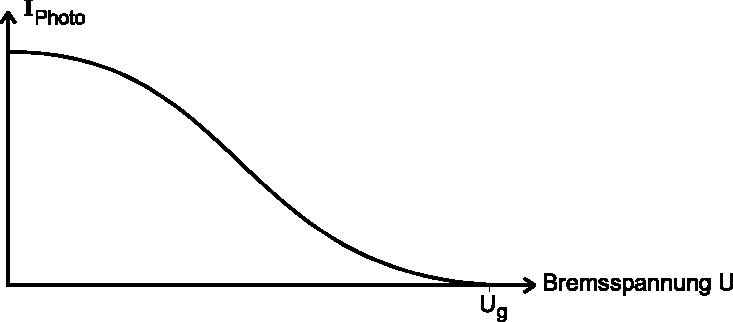
\includegraphics{figures/Abb4.pdf}
    \caption{Photostrom $I_\text{Photo}$ in Abhängigkeit der Bremsspannung $U$ \,\cite{ap10}.}
    \label{fig:abb4}
\end{figure}

Dabei besteht zwischen Photostrom und Bremsspannung unter bestimmten Voraussetzungen ein quadratischer Zusammenhang.
\begin{equation*}
    I_{Ph} \sim U^2 \,.
\end{equation*}

Sollte der Fall auftreten, dass zwar $h \, \nu \geq A_\text{k}$, allerdings nicht $h \, \nu \geq A_\text{A}$ ist, tritt kein Photostrom auf, da die Elektronen gegen ein Gegenfeld anlaufen müssten,
um die Anode zu erreichen.


So muss zunächst ein beschleunigendes Potential $U_\text{b}$ angelegt werden, sodass bei
\begin{equation*}
    h \, \nu + \text{e}_0 \, U_\text{b} \geq A_\text{A}
\end{equation*}
erneut ein Photostrom gemessen werden kann.

%%% Theorie Ende
